\chapter{Praktischer Teil}
\label{chapter_Praktischer_Teil}
In diesem Kapitel werden die verschiedenen Sensorschaltungen und deren Konfiguration, die Problem
die sich bei der Realisierung ergaben, sowie die Ergebnisse und Auswertungen beschrieben. Außerdem werden die verschiedenen Möglichkeiten zur Datenspeicherung und Visualisierung dargestellt und erklärt. Am Anfang dieses Kapitels werden die zur Realisierung der verschiedenen Aufgaben benötigten Bauteile, kurz etwas näher erklärt und aufgelistet. In Abschnitt \ref{section_DS18S20} wird eine Schaltung mit einem einzigen 1-Wire Temperatursensor aufgebaut, bei der zweiten Schaltung in Abschnitt \ref{section_HTY221} kommt zu dem Sensor aus \ref{section_DS18S20} ein zweiter Temperatursensor und ein Sensor zur Temperaturmessung und Bestimmung der Luftfeuchtigkeit hinzu. Der letzte Abschnitt (\ref{section_BMA020}) befasst sich mit der Realisierung einer Vibrationsmessung mittels Beschleunigungssensors.

\section{Benötigte Materialien}
\label{section_Benötigte_Materialien}
Die in Tabelle aufgelisteten Materialien wurden für die in Kapitel \ref{chapter_Praktischer_Teil} beschriebenen Versuche verwendet. In den jeweiligen Abschnitten, werden die  einzelnen Sensoren mit deren wichtigsten Technischen Daten noch genauer erklärt. 

%Tabelle 1
\begin{table}[H]
%\rowcolors{2}{black!10}{black!20}
\centering
\begin{tabular}{
lc
}
\toprule
\multicolumn{1}{p{6cm}}{\textit{Bezeichnung}} & \multicolumn{1}{p{3.5cm}}{\centering\textit{Anzahl} } \\\midrule
Raspberry Pi\,3& 1 \\
&\\
Temperatursensor DS18S20 & 2 \\
&\\
Sensor HYT\,221 & 1\\
&\\
3-Achsen-Beschleunigungssensor & 1\\
&\\
Drahtbrücken & mehrere\\
&\\
elektrischer Widerstand 4.7\,$k\Omega$ & 1\\
&\\
Elektronik Steckbrett & 1\\
\bottomrule
\end{tabular}
\caption{benötigte Materialien}
\label{Tabelle_benötigte_Materialien}
\end{table}

%Abschnitt DS18S20
\section{Temperaturmessung mit Sensor DS18S20}
\label{section_DS18S20}
Abschnitt \ref{section_DS18S20} befasst sich mit dem Schaltungsaufbau zur Temperaturmessung mittels DS18S20. Weiterhin werden die verschiedenen Möglichkeiten zur Datenspeicherung (RRD Tool, mySQL), sowie eine Möglichkeit zur Visualisierung der Daten erläutert. 
 



\subsection{DS18S20}
\label{subsection_DS18S20}
Der DS18S20 (siehe Abbildung \ref{Abb_DS18S20}) ist ein digitaler 1-Wire Temperatursensor, der eine 9\,Bit Temperaturmessung ermöglicht. Dieser ist von der Firma \textit{Maxim Integrated} entwickelt worden.
Folgend werden die wichtigsten technischen Daten des DB18S20 aufgeführt.

%Abbildund Daten DS18S20
\begin{figure}[!h] 
  \centering
     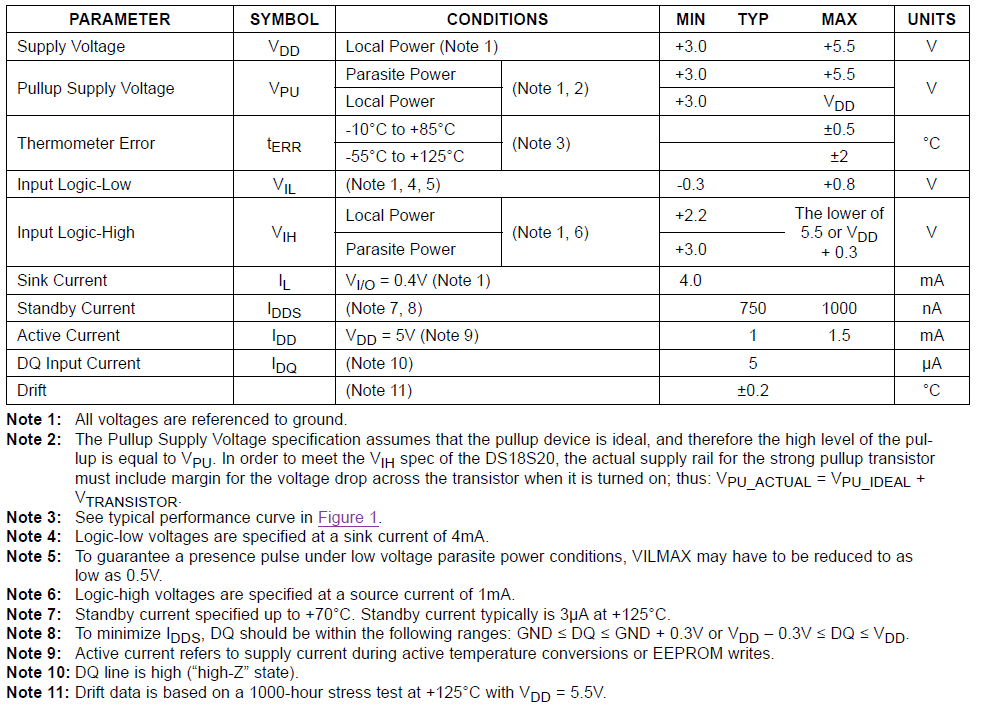
\includegraphics[scale=.6]{BilderAllgemein/Daten_DB18S20.png}
  \caption{elektische Daten DB18S20 \citep[S. 2]{Datenblatt_DB18S20}}
  \label{Abb_elektrische_Daten_DS18S20}
\end{figure}

%Abbildund  DS18S20
\begin{figure}[!h] 
  \centering
     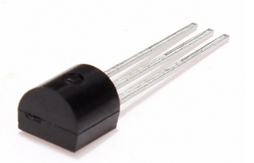
\includegraphics[scale=.4]{BilderAllgemein/DS18S20.png}
  \caption{DS18S20 \citep{Bild_DS18S20}}
  \label{Abb_DS18S20}
\end{figure}

\subsection{Schaltungsaufbau}
\label{subsection_Schaltungsaufbau_DS18S20}

Abbildung \ref{Abb_Schaltung_DS18S20} zeigt den schematischen Schaltungsaufbau mit dem Temperatursensor DS18S20. Anzumerken ist, dass die in der Schaltung in Abbildung \ref{Abb_Schaltung_DS18S20} dargestellten Bauteile optisch nicht immer den realen Bauteilen entsprechen (z.B. Aufdruck auf dem Sensor). Die Beschaltung der Bauteile wurde in der praktischen Erprobung ganz genau so durchgeführt. 

%Abbildund Schaltungsaufbau DS18S20
\begin{figure}[!h] 
  \centering
     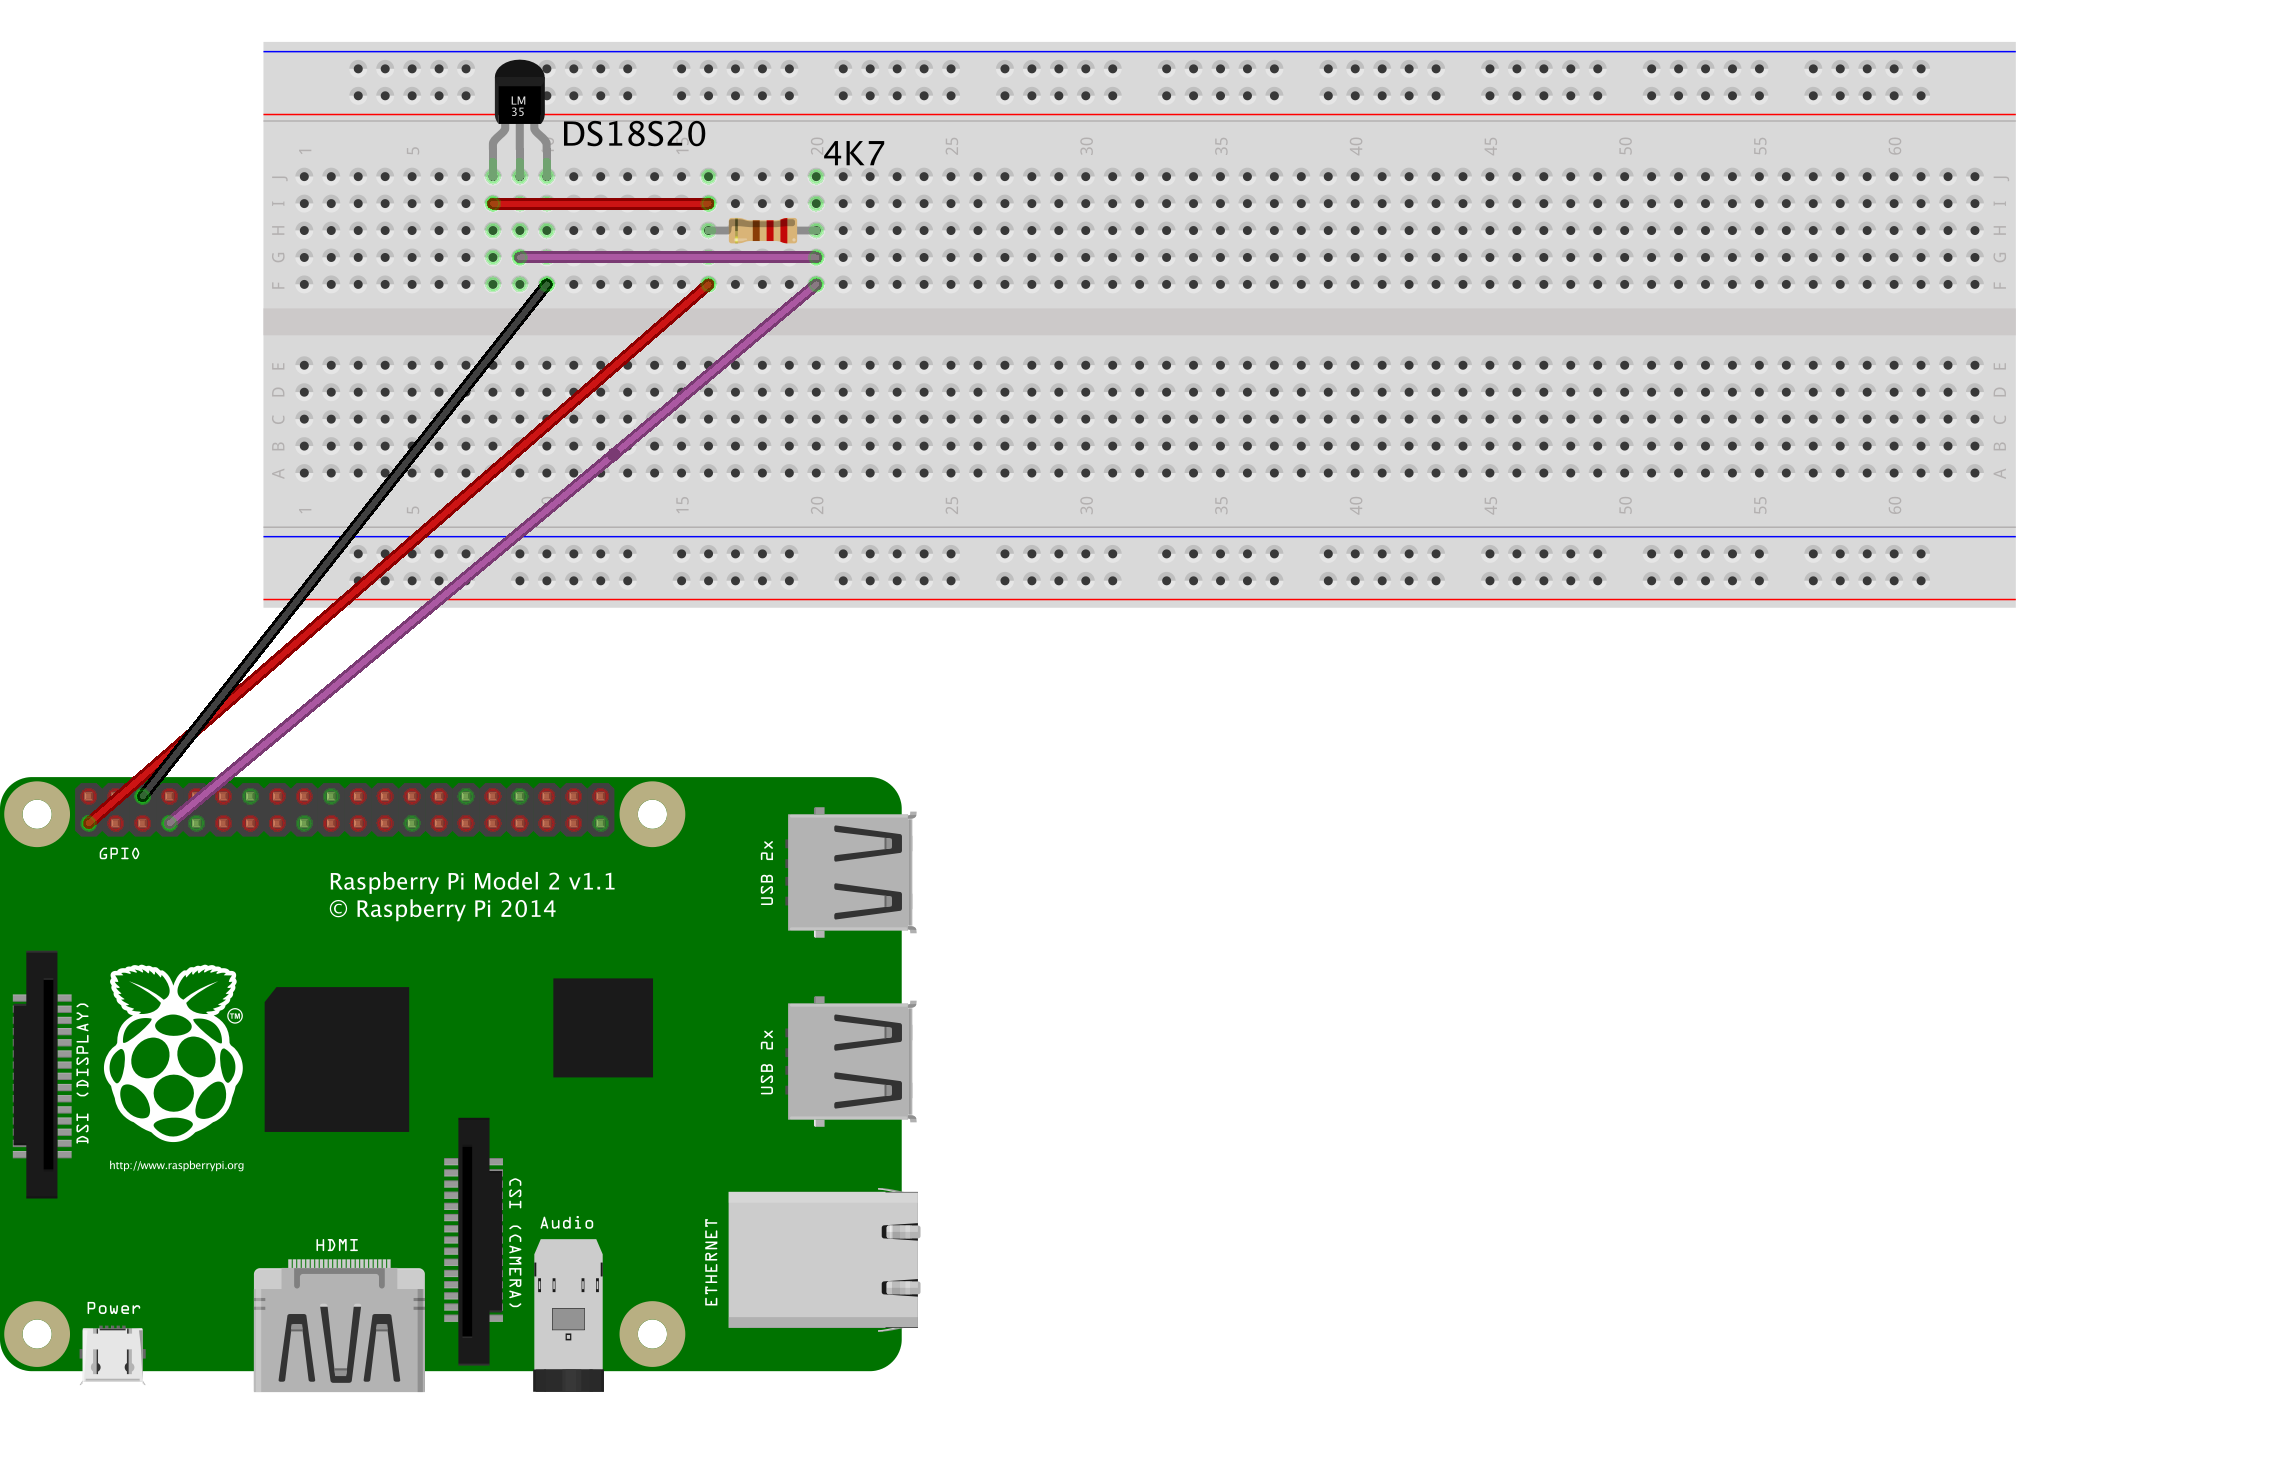
\includegraphics[scale=.8]{BilderAllgemein/Schaltung_DS18S20.png}
  \caption{Schaltungsaufbau DS18S20}
  \label{Abb_Schaltung_DS18S20}
\end{figure}

Die oben dargestellte Schaltung\footnote{gezeichnet mit Fritzing} zur Temperaturmessung wird folgendermaßen realisiert, der Pin $V_{DD}$ des Sensors ist mit Pin\,1 (3,3\,V) des \ac{RPI}\,3 verbunden (rote Verbindung). Die schwarze Verbindung stellt die GROUND Verbindung des Pin\,6 des \ac{RPI} mit dem GND Pin des Sensors dar. Weiterhin ist der er DQ Pin des Sensors (1-Wire Interface) mit dem Pin\,7 des \ac{RPI} verbunden (violette Verbindung) welcher für den 1-Wire Bus verwendet wird. Zu dem  $V_{DD}$ Pin  und dem DQ Pin ein Pullup Widerstand parallel geschalten.

\subsection{Auslesen des Sensors}
\label{subsection_Auslesen_DS18S20}
Um die vom Sensor erfassten Daten auf dem \ac{RPI}\,3 auszulesen, wird ein Python Script verwendet. Dieses wird im Anschluss an Hand kurzer Ausschnitte aus dem Quellcodes erklärt. Der komplette Quellcode ist im Anhand dieser Arbeit zu finden.\\

%Quellcode DS18S20
\lstset{escapeinside={\%*}{*},numbers=left,stepnumber=1}
\lstinputlisting[language=Python, firstline=16, lastline=32, caption=Auslesen der gemessenen Temperatur, label=list:Quellcode_DS18S20]{Listings/DS18S20/DS18S20.py}

Um die Temperatur des Sensors auslesen zu können wird als erstes das File wie in Zeile 2 des Codes ersichtlich ist geöffnet und dessen Inhalt in eine Variable gespeichert. Dieses File enthält die gesamten an den \ac{RPI}\,3 angeschlossenen IDs der 1-Wire Sensoren. Jeder angeschlossenen 1-Wire Sensor besitzt im Pfad \texttt{/sys/bus/w1/devices/} einen Ordner mit seiner ID. In diesem gibt es wiederum eine Datei mit der Bezeichnung \texttt{w1\_slave}, die die gemessenen Daten enthält. Um diese auszulesen, werden in unseren Python Script in den Zeilen $8-15$ verschiedene Schritte durchgeführt, auf die nicht näher eingegangen wird\footnote{kann in verschiedenen Python Tutorials nachgelesen werden}. Da die Temperatur in dieser Datei vom Sensor im Format von z.B. 17687 ($\approx$ 17,7 $^\circ$C) angegeben wird, muss dieser Wert noch durch 1000 dividiert werden um den genauen Temperaturwert zu erhalten(Zeile 15 im Quellcode). In Zeile 16 wird der Wert noch auf zwei Stellen nach dem Komma gerundet und ist in der Variable \texttt{temperature} gespeichert. Mit dem Wert dieser Variable kann nun weiter gearbeitet werden.

%Subsection Datenspeicherung
\subsection{Speicherung der Daten}
\label{subsectio_Datenspeicherung_DS18S20}
Wie schon in Abschnitt \ref{section_DS18S20} angesprochen, wird in dieser Arbeit auf zwei verschiedene Möglichkeiten der Datenspeicherung eingegangen. Zum Einen mit dem RRDtool und zum Andern mittels mySQL Datenbank. Die Möglichkeit der Datenspeicherung in einer mySQL Datenbank wird im Abschnitt \ref{section_HTY221} beschrieben. In diesem Abschnitt wird näher auf die Möglichkeiten mit dem RRDtool eingegangen.

\subsection*{RRDtool}
Unter dem RRDtool versteht man ein Programm, welches es ermöglicht, Messdaten für einen beim Erstellen festgelegten Zeitbereich zu speichern. RRD steht für \textit{Round-Robin-Database}, diese wird durch das Tool in einer Datei erzeugt, die von der Erstellung weg eine feste Größe besitzt. Dies ist ein großer Unterschied zu herkömmlichen mySQL Datenbanken, da bei diesen mit zunehmender Zeit und Datenmenge auch die Größe der Datenbank immer mit anwächst. Das Anwachsen der Größe der Datei wird bei der RRD Datenbank dadurch verhindert, dass sie wie ein Ringbuffer arbeitet. Dies bedeutet, dass wenn der Speicherplatz belegt ist, Werte zusammengefasst (z.B. durch Bildung eines Mittelwertes für einen Tag aus den einzelnen stündlichen Werten) und die ältesten überschrieben werden. Somit kann sichergestellt werden, dass die Größe der Datenbank schon beim Erstellen dieser festgelegt ist.\\
Wie eine solche Datenbank definiert und erstellt wird, wird im Quellcode beschrieben. Zum Erstellen der Datenbank wurde ein Shell-Script verwendet um nicht jedes Mal wenn die Datenbank neu erstellt wird alle Befehle einzeln eingeben zu müssen.

%Quellcode DS18S20
\lstset{escapeinside={\%*}{*},numbers=left,stepnumber=1}
\lstinputlisting[language=Python, firstline=1, lastline=9, caption=Erstellung RRD Datenbank , label=list:Quellcode_RRD_Datenbank]{Listings/DS18S20/RRD_DB_Erstellen.sh}
















\newpage
%Abschnitt HYT-221
\section{Temperatur- und Luftfeuchtigkeitsmessung mit HTY-221}
\label{section_HTY221}

\subsection{HYT-221}
\label{subsection_HYT221}
Der HYT-221 ist ein Sensor zur Messung der Temperatur und Luftfeuchtigkeit. Er wurde von der Schweizer Firma \ac{IST} für die Anwendung in den Bereichen Meteorologie, Industrielle Trocknungstechnik, Medizinische Geräte, Luftfahrt und Extremsport entwickelt. Der Sensor kommuniziert über eine \ac{I$^2$C} Schnittstelle und besitzt eine hohe Messgenauigkeit. In Tabelle \ref{Tabelle_Technische_Daten_HYT221}  werden die wichtigsten Daten des Sensors aufgelistet. Diese wurden dem Sensor zugehörigen Datenblatt entnommen \citep{Datenblatt_HYT221}.

%Tabelle Technische Daten HYT-221
\begin{table}[H]
%\rowcolors{2}{black!10}{black!20}
\centering
\begin{tabular}{
llll
}
\toprule
\multicolumn{2}{p{7cm}}{\centering\textbf{Feuchtemessung}} & \multicolumn{2}{p{7cm}}{\centering\textbf{Temperaturmessung} } \\
\multicolumn{1}{p{4cm}}{\textit{Bezeichnung}} & \multicolumn{1}{p{3cm}}{\centering\textit{Werte} }&\multicolumn{1}{p{4cm}}{\textit{Bezeichnung}} & \multicolumn{1}{p{3cm}}{\centering\textit{Werte} }\\\midrule
Messbereich & 0\dots 100\,\% rF & Messbereich  & -40\dots +125 $^\circ\text{C}$ \\
&&&\\
Genauigkeit & $\pm$ 1,8\,\% rF& Genauigkeit & $\pm$ 0,2 $^\circ\text{C}$\\
&&&\\
Auflösung & 0,02\,\% rF & Auflösung & 0.015 $^\circ\text{C}$\\
\bottomrule
\end{tabular}
\caption{Technische Daten HYT-221 \citep{Datenblatt_HYT221}}
\label{Tabelle_Technische_Daten_HYT221}
\end{table}

Für einen sicheren Betrieb des Sensors muss die angelegte Versorgungsspannung zwischen 2,7\dots 5,5\,$V$ liegen.

%Abbildund  HYT221
\begin{figure}[!h] 
  \centering
     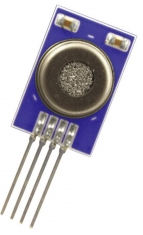
\includegraphics[scale=.8]{BilderAllgemein/HYT221.png}
  \caption{HYT-221 \citep{Bild_HYT221}}
  \label{Abb_HYT221}
\end{figure}




\section{Vibrationsmessung mit Sensor BMA020}
\label{section_BMA020}